\documentclass[landscape,twocolumn,a4paper]{article}
\usepackage[utf8x]{inputenc}
\usepackage[ngerman]{babel}
\usepackage{listings}
\usepackage{babel}

\usepackage[T1]{fontenc}
\usepackage{booktabs} % schöne Tabellen
\usepackage{graphicx}
\usepackage{csquotes} % Anführungszeichen
\usepackage{paralist} % kompakte Aufzählungen
\usepackage{amsmath,textcomp,tikz} %diverses
\usepackage{eso-pic} % Bilder im Hintergrund
\usepackage{mdframed} % Boxen
\usepackage{multirow}
\usepackage{amssymb}

\usepackage{mathtools}
\usepackage[top=20mm,left=10mm,right=10mm,bottom=10mm]{geometry}
\usepackage{fancyhdr}
\pagestyle{fancy}
\fancyhead[L]{Lösungen zu Zahlentheorie/Kryptographie}
\fancyhead[R]{\thepage}
\fancyfoot{}

\lstset{language=Python, tabsize=4, basicstyle=\footnotesize, showstringspaces=false, mathescape=true}
\lstset{literate=%
  {Ö}{{\"O}}1
  {Ä}{{\"A}}1
  {Ü}{{\"U}}1
  {ß}{{\ss}}1
  {ü}{{\"u}}1
  {ä}{{\"a}}1
  {ö}{{\"o}}1
}
\begin{document}
\newcommand{\ggT}{\operatorname{ggT}}
\newcommand{\Mod}[3]{#1\equiv#2\text{ mod }#3}
\newcommand{\tmod}{\text{ mod }}
\newcommand\x{1}
\newcounter{y}
\setcounter {y} {1}

\parindent 0mm

\textbf{Diophantische Gleichungen} 
\bigskip

\textbf{A\arabic {y}:}   \\
Zerlege die Zahlen in Primfaktoren und bestimme damit den ggT. Bestimme dann nochmal den ggT mit
dem Euklidschen Algorithmus. \\
a.  $a = 315, b=693$ \quad b. $a=336,b=264$
\bigskip  \stepcounter{y}

Lösung: \\
a. Primfaktorzerlegung: $315 = 3 \cdot 3 \cdot 5 \cdot 7, \quad 693 = 3 \cdot 3 \cdot 7 \cdot 11 \\ \Rightarrow \ggT(315,693) = 3 \cdot 3 \cdot 7 = 63$. Euklidscher Algorithmus: 
\begin{lstlisting}
   693    315
   315     63
    63      0
\end{lstlisting}

b. Primfaktorzerlegung: $336 = 2 \cdot 2 \cdot 2 \cdot 2 \cdot 3 \cdot 7, \quad 264 = 2 \cdot 2 \cdot 2 \cdot 3 \cdot 11  \\ \Rightarrow \ggT(336,264) = 2 \cdot 2 \cdot 2 \cdot 3= 24$. Euklidscher Algorithmus: 
\begin{lstlisting}
   336    264
   264     72
    72     48
    48     24
    24      0
\end{lstlisting}

 

\textbf{A\arabic {y}:}   \\
Berechne mit dem Euklidischen Algorithmus: \\
a.  $\ggT(150,54)$ \quad b. $\ggT(300,468)$ \quad 
 c.$\ggT(44,18)$ \quad d. $\ggT(992,999)$
\bigskip \stepcounter{y}

Lösung: \\

\begin{minipage}[t]{4cm}
a.
\begin{lstlisting}
   150     54
    54     42
    42     12
    12      6
     6      0
\end{lstlisting}
$\ggT(150,54) = 6$ 
\end{minipage}
\begin{minipage}[t]{4cm}
b.
\begin{lstlisting}
   468    300
   300    168
   168    132
   132     36
    36     24
    24     12
    12      0
\end{lstlisting}
$\ggT(300,468) = 12$ 
\end{minipage}
\begin{minipage}[t]{4cm}
c.
\begin{lstlisting}
    44     18
    18      8
     8      2
     2      0
\end{lstlisting}
$\ggT(44,18) = 2$ 
\end{minipage}
\begin{minipage}[t]{4cm}
d.
\begin{lstlisting}
   999    992
   992      7
     7      5
     5      2
     2      1
     1      0
\end{lstlisting}
$\ggT(992,999) = 1$ 
\end{minipage}


 
\textbf{A\arabic {y}:}   \\
Berechne den ggT der Zahlen $a$ und $b$ und stelle ihn in der Form $ax + by$ dar. \\
a.   $ a = 531, b = 93$  \quad b. $ a = 753, b = 64$
\bigskip \stepcounter{y}

Lösung: \\
a. 
\begin{lstlisting}
    a    b    q    r    x    y
  531   93    5   66   -7   40
   93   66    1   27    5   -7
   66   27    2   12   -2    5
   27   12    2    3    1   -2
   12    3    4    0    0    1
\end{lstlisting}
$\ggT(531,93) = 3 = 531 \cdot  -7 + 93  \cdot 40$ \\

b. 
\begin{lstlisting}
    a    b    q    r    x    y
  753   64   11   49   17 -200
   64   49    1   15  -13   17
   49   15    3    4    4  -13
   15    4    3    3   -1    4
    4    3    1    1    1   -1
    3    1    3    0    0    1

753 * 17 + 64 * -200 = 1
\end{lstlisting}
$\ggT(753,64) = 1  =753 \cdot 17 + 64 \cdot -200$ \\
 

\textbf{A\arabic {y}:}   \\
Bestimme - falls möglich - eine Lösung $(x/y)$ der angegebenen Gleichung: \\
a.  $96x+66y=6$ \quad b. $96x+66y=18$ \\
c.  $119x+143y=4$ \quad d. $91x+35y=12$.
\bigskip \stepcounter{y}
 
 Lösung: \\
 a. Division durch 6 ergibt $16x+11y=1$. Eine Lösung ist offenbar $(-2/3)$. \\
 b. Aus a. folgt als eine Lösung: $(-6/9)$. \\
 c. 
 \begin{lstlisting}
    a    b    q    r    x    y
  143  119    1   24    5   -6
  119   24    4   23   -1    5
   24   23    1    1    1   -1
   23    1   23    0    0    1
\end{lstlisting} Es gilt: $119 \cdot  -6 + 143 \cdot 5 = 1$. Also ist eine Lösung $(-24/20)$ \\
d. $\ggT(91,35) = 7 \nmid 12 \Rightarrow$ Die Gleichung hat keine Lösung. \\

 \textbf{A\arabic {y}:}   \\
Vereinfache die Gleichung und finde möglichst viele Lösungen: \\
a.   $42x+126y=84$ \quad b. $81x+54y=27$ \quad 
 c. $77x+121y=44$ 
 \bigskip \stepcounter{y}
 
 Lösung: \\
 a. Division durch 42 ergibt: $x + 3y = 2$. $(2/0)$ ist eine Lösung. Weitere Lösungen: $(2+3k/-k)$ für $k \in \mathbb{Z}$. \\
 b. Division durch 27 ergibt: $3x + 2y = 1$. $(1/-1)$ ist eine Lösung. Weitere Lösungen: $(1+2k/-1-3k)$ für $k \in \mathbb{Z}$. \\
 c. Division durch 11 ergibt: $7x + 11y = 4$. $(-1/1)$ ist eine Lösung. Weitere Lösungen: $(-1+11k/1-7k)$ für $k \in \mathbb{Z}$. \\



 
 \textbf{Kongruenzen} \bigskip
 
 \textbf{A\arabic {y}:}   \\
Berechne den Elferrest von 200, 500, 700, 1000 und 1000000. \\

Lösung: \\
$200 \equiv 110 + 88 + 2 \equiv 2 \tmod 11$ \\
$500 \equiv 200 + 200 + 99 + 1 \equiv 2 + 2+ 1 \equiv 5 \tmod 11$ \\
$700 \equiv 200 + 500 \equiv 2 + 5 \equiv 7 \tmod 11$ \\
$1000 \equiv 500 + 500 \equiv 5 + 5 \equiv 10 \tmod 11$ \\
$1000000 \equiv 1000 * 1000 \equiv -1 \cdot -1 \equiv 1 \tmod 11$ \\

Die Elferreste sind 2, 5, 7, 10, 1.
\bigskip \stepcounter{y}
 
 \textbf{A\arabic {y}:}   \\
Berechne:
a. $(34 + 97) \tmod 3$ \quad b. $(-13-25) \tmod 4$ \quad c. $(587 + 5 457 803) \tmod 5$ \\
d. $(15 \cdot 91) \tmod 11$  \quad e. $(658 \cdot 49) \tmod 7$ \quad f. $(12508 \cdot 5093) \tmod 10$ \\
g. $7^3\tmod 3$  \quad h. $5^{100}\tmod 4$ \quad i. $5^{100}\tmod 6$
\bigskip \stepcounter{y}

Lösung: \\
a.  $34 + 97 \equiv 1 + (-2) \equiv -1 \equiv 2 \tmod 3 $ \\
b.  $-13-25  \equiv -38 \equiv 2 \tmod 4$ \\
c.  $587 + 5 457 803 \equiv 2 + 3 \equiv 5 \equiv 0 \tmod 5$ \\
d.  $15 \cdot 91 \equiv 4 \cdot 3 \equiv 12 \equiv 1 \tmod 11$\\
e. $658 \cdot 49 \equiv 658 \cdot 0 \equiv 0 \tmod 7$ \\
 f. $12508 \cdot 5093 \equiv 8 \cdot 3 \equiv 24 \equiv 4 \tmod 10$ \\
 g. $7^3 \equiv 1^3 \equiv 1 \tmod 3$ \\
 h. $5^{100} \equiv 1^{100} \equiv 1 \tmod 4$ \\
 i. $5^{100}\equiv (-1)^{100} \equiv 1 \tmod 6$
 
 
\textbf{A\arabic {y}:}   \\
Berechne: a. $2^2, 2^4, 2^8, 2^{12}, 2^{100} \tmod 100$. \quad b. $2^4,2^{20},2^{100},2^{1001} \tmod 5$. \\
c. $2^3, 2^{20}, 2^{100} \tmod 7$ \quad d. $3^{20} \tmod 5$
\bigskip \stepcounter{y}

Lösung: \\
a. $2^2 \equiv 1, 2^4 \equiv (2^2)^2 \equiv 1, 2^8 \equiv (2^4)^2 \equiv 1, 2^{12} \equiv (2^4)^3 \equiv 1, 2^{100} = (2^2)^{50}\equiv 1 \tmod 3$ \\
b. $2^4 \equiv 16 \equiv 1, 2^{20} \equiv (2^4)^5 \equiv 1, 2^{100} \equiv (2^{20})^5 \equiv 1, 2^{1001} \equiv 2 \cdot 2^{1000} \equiv 2 \cdot (2^{100})^{10} \equiv 2 \tmod 5$ \\
c $2^3 \equiv 1, 2^{20} \equiv 2^ {18} \cdot 2^2 \equiv 1 \cdot 4 \equiv 4, 2^{100} \equiv (2^{20})^5 \equiv
4^5 \equiv 4^2 \cdot 4^2 \cdot 4 \equiv 2 \cdot 2 \cdot 4 \equiv 2 \tmod 7$ \\
d.  $3^{20} \equiv (3^2)^{10} \equiv (-1)^{10} \equiv 1 \tmod 5$ \\

\textbf{A\arabic {y}:}   \\
a. Untersuche, welchen Rest Quadratzahlen modulo 10 haben können. \\
b. Zeige, dass 25036008 keine Quadratzahl sein kann.
\bigskip \stepcounter{y}

Lösung: \\
a. $0^2 \equiv 0, 1^2 \equiv 1, 2^2 \equiv 4, 3^2 \equiv 9, 4^2 \equiv 6, 5^2 \equiv 5, 6^2 \equiv 6, 7^2 \equiv 9,
8^2 \equiv 4, 9^2 \equiv 1 \tmod 10$. Quadratzahlen habe modulo 10 die Reste 0,1,4,5,6 oder 9. \\
b. $25036008 \equiv 8 \tmod 10$, kann also nach a. keine Quadratzahl sein. \\

\textbf{A\arabic {y}:}   \\
Wende die Teilbarkeitsregeln für 2-12 auf folgende Zahlen an:\\
a. 1540 \quad b. 1623272 \quad c. 13678500 \quad d. 123456789
\bigskip \stepcounter{y}

Lösung: \\
(QS = Quersumme, aQS = alternierende Quersumme, 7R = 7er Regel) \\
a. QS = 10, aQS = 0, $4 \mid 40, 8 \nmid 140$, 7R: 54 7 $\Rightarrow$
1540 teilbar durch 2 4 5 7 10 11.\\
b. QS = 23, aQS = -9, $4 \mid 72, 8 \mid 272$, 7R: 162323 16226 1610 161 14 $\Rightarrow$
1623272 teilbar durch 2 4 7 8. \\
c. QS = 30, aQS = 0, $4 \mid 00, 8 \nmid 500$, 7R: 1367850 136785 13668 1350 135 3 $\Rightarrow$
13678500 teilbar durch 2 3 4 5 6 10 11 12.\\
c. QS = 45, aQS = 5, $4 \nmid 89$, 7R: 12345660 1234566 123444 12336 1221 120 12 $\Rightarrow$
123456789 teilbar durch 3 9. \\

\textbf{A\arabic {y}:}   \\
Begründe, dass folgende Teilbarkeitsregeln falsch sind: \\
a. Eine Zahl ist genau dann durch 8 teilbar, wenn die aus ihren letzten beiden Ziffern gebildete Zahl durch 8 teilbar ist. \\
b. Eine Zahl ist genau dann durch 24 teilbar, wenn sie durch 4 und durch 6 teilbar ist. \\
c. Eine Zahl ist genau dann durch 4 teilbar, wenn ihre Quersumme durch 4 teilbar ist.
\bigskip \stepcounter{y}

Lösung: \\
a. Gegenbeispiel: $116 \equiv 4 \tmod 8$ \\
b. Gegenbeispiel: 12 \\
c. Gegenbeispiel: 22 \\


\textbf{A\arabic {y}:}   \\
Bestimme möglichst alle ganzzahligen Lösungen $x$ der folgenden
  Gleichungen: \\
a. $\Mod{5+x}{2}{7}$\quad b.   $\Mod{5\cdot x}{2}{7}$ \\ 
c. $\Mod{5\cdot x}{2}{10}$  \quad d.  $\Mod{-34}{x}{5}$
\bigskip \stepcounter{y}

Lösung: 
\begin{minipage}[t]{4cm}
\begin{align*}
a. \quad 5 + x &\equiv 2 \tmod 7 \\
x &\equiv -3 \tmod 7 \\
x &\equiv 4 \tmod 7 \\
\mathbb{L} &= \{4 +7k \mid k \in \mathbb{Z}\}
\end{align*}  
\end{minipage} 
\begin{minipage}[t]{4cm}
\begin{align*}
b. \quad 5 x &\equiv 2 \tmod 7 \\
5x + 7y &= 2  \quad  (-1,1) \text{ ist Lösung} \\
\mathbb{L} &= \{-1 +7k \mid k \in \mathbb{Z}\}
\end{align*}  
\end{minipage} 

\begin{minipage}[t]{4cm} 
\begin{align*}
c. \quad 5 x &\equiv 2 \tmod 10 \\
5x + 10y &= 2  \quad  \text{Es gilt: }\ggT(5,10) \nmid 2 \\
\mathbb{L} &= \{ \}
\end{align*}  
\end{minipage} 
\begin{minipage}[t]{4cm} 
\begin{align*}
d. \quad -34&\equiv x \tmod 5 \\
x & \equiv 1 \tmod 5 \\
\mathbb{L} &= \{1 + 5k \mid k \in \mathbb{Z} \}
\end{align*}  
\end{minipage} \\


\textbf{A\arabic {y}:}   \\
Beweise die folgenden Aussagen:\\
a. Wenn $\Mod{a}{b}{m}$ und $\Mod{c}{d}{m}$, dann
    $\Mod{a+c}{b+d}{m}$. \\
b. Wenn $\Mod{a}{b}{m}$, dann $\Mod{-a}{-b}{m}$. \\
c. Wenn $\Mod{a}{b}{m}$ und $\Mod{b}{c}{m}$, dann
    $\Mod{a}{c}{m}$.
\bigskip \stepcounter{y}

Lösung: \\
a. Nach Voraussetzung gilt $a \equiv b \tmod m$ und $c \equiv d \tmod m$, d.h. es gibt $k_1, k_2 \in 
\mathbb{Z}$ mit $a = b + k_1m$ und $c = d + k_2m$. Daraus  ergibt sich: $a + c = b + d + (k_1 + k_2)m$ und 
dies bedeutet $a + c \equiv b +d \tmod m$. \hfill $\square{}$ \\
b. Nach Voraussetzung gilt $a \equiv b \tmod m$, d.h. es gibt ein $k \in \mathbb{Z}$ mit: $a = b + km$. Damit 
gilt auch $-a = -b - km$. Setze $k_1 = -k$, dann gilt also $-a = -b + k_1m$ mit $k_1 \in \mathbb{Z}$.
Das bedeutet $-a \equiv -b \tmod m$. \hfill $\square{}$ \\
c. Nach Voraussetzung gilt $a \equiv b \tmod m$ und $b \equiv c \tmod m$, d.h. es gibt $k_1, k_2 \in 
\mathbb{Z}$ mit $a = b + k_1m$ und $b = c + k_2m$. Daraus ergibt sich $a =c + k_2m + k_1m = c +(k_2+k_1)m$.
Das bedeutet $a \equiv c \tmod m$. \hfill $\square{}$ \\

 \textbf{Restklassen} \bigskip

\textbf{A\arabic {y}:}   \\
Bestimme mit dem erweiterten Euklidschen Algorithmus: \\
 a.  $\dfrac{\overline{5}}{\overline{33}}$ in  $\mathbb{Z}_{37}$. \quad
 b.  $\dfrac{\overline{7}}{\overline{20}}$ in  $\mathbb{Z}_{89}$.
\bigskip \stepcounter{y}

Lösung: \\
a.
\begin{lstlisting}
    a    b    q    r    x    y
   37   33    1    4   -8    9
   33    4    8    1    1   -8
    4    1    4    0    0    1

37 * -8 + 33 * 9 = 1
\end{lstlisting}   
Also gilt: $\dfrac{\overline{1}}{\overline{33}} = \overline{9}$. Daraus folgt: $\dfrac{\overline{5}}{\overline{33}} =  \overline{45} = \overline{8}$ in  $\mathbb{Z}_{37}$.

 
b.
\begin{lstlisting}
    a    b    q    r    x    y
   89   20    4    9    9  -40
   20    9    2    2   -4    9
    9    2    4    1    1   -4
    2    1    2    0    0    1

89 * 9 + 20 * -40 = 1
\end{lstlisting}   
Also gilt: $\dfrac{\overline{1}}{\overline{20}} = \overline{-40}$. Daraus folgt: $\dfrac{\overline{7}}{\overline{20}} =  \overline{-280} = \overline{76}$ in  $\mathbb{Z}_{89}$. \\

\textbf{A\arabic {y}:}   \\
Bestimme mit dem kleinen Satz von Fermat: \\
 a.  $\overline{4}^{-11}$ in  $\mathbb{Z}_{13}$. \quad
 b.  $\overline{6}^{31}$ in  $\mathbb{Z}_{29}$. \quad
 c.  $ \overline{6}^{32}$ in  $\mathbb{Z}_{29}$. 
\bigskip \stepcounter{y}

Lösung: \\
a. $\overline{4}^{-11}$ = $\overline{4}^{12} \cdot \overline{4}^{-11} = \overline{4}$ in  $\mathbb{Z}_{13}$. \\
b. $\overline{6}^{31} =  \overline{6}^{28} \cdot  \overline{6}^{3} = \overline{36} \cdot \overline{6} = \overline{42} =  \overline{13} \text{ in } \mathbb{Z}_{29}$. \\
 c.  $ \overline{6}^{32} =  \overline{13} \cdot  \overline{6} =  \overline{78} =  \overline{20}$ in  $\mathbb{Z}_{29}$.\\ 

\textbf{A\arabic {y}:}   \\
Berechne in $\mathbb{Z}_{23}$ die folgenden Brüche: \\
a.  $\dfrac{\overline{1}}{\overline{5}^{21}} $ \quad
b.  $\dfrac{\overline{1}}{\overline{10}^{13}} $ \quad
c.  $\dfrac{\overline{7}}{\overline{10}^{12}} $ \quad
d.  $\dfrac{\overline{7}}{\overline{22}} $ 
\bigskip  \stepcounter{y}

Lösung: \\
a.  $\dfrac{\overline{1}}{\overline{5}^{21}}  = \overline{5}^{-21} = \overline{5}^{22-21} = \overline{5}$ \\
b. $\dfrac{\overline{1}}{\overline{10}^{13}} =  \overline{10}^{22-13} =  \overline{10}^{9} = \overline{10}^{8+1}
=   \overline{2} \cdot \overline{10}= \overline{20}$ \quad $(10^2, 10^4,10^8 \equiv 8,-5,2)$ \\
c.  $\dfrac{\overline{7}}{\overline{10}^{12}} = \overline{7} \cdot \overline{10}^{22-12} = \overline{7} \cdot \overline{10}^{8+2} =  \overline{7} \cdot \overline{2} \cdot \overline{8} = \overline{20}$   \\
d.  $\dfrac{\overline{7}}{\overline{22}} = \dfrac{\overline{7}}{\overline{-1}} =  \overline{-7} = \overline{16}$  \\

 
\textbf{A\arabic {y}:}   \\
Prüfe, ob die angegebene Zahl eine Primitivwurzel ist: \\
 a. 4 in  $\mathbb{Z}_{13}$ \quad  b. 6 in  $\mathbb{Z}_{13}$
\bigskip \stepcounter{y}

 Lösung: \\
a.  $4^1 \equiv 4, 4^2 \equiv 16 \equiv 3, 4^3 \equiv 12, 4^4 \equiv 9, 4^5 \equiv 36 \equiv 10, 4^6 \equiv 40 \equiv 1 \tmod 13 \Rightarrow$ 4 ist keine Primitivwurzel in  $\mathbb{Z}_{13}$. \\
b. $6^1 \equiv 6,  6^2 \equiv 36 \equiv 10, 6^3 \equiv 60 \equiv 8, 6^4 \equiv 48 \equiv 9,  6^5 \equiv 54 \equiv 2,  
6^6 \equiv 12,   6^7 \equiv 20 \equiv 7,   6^8 \equiv 16 \equiv 3,   6^9 \equiv 18 \equiv 5,  6^{10} \equiv 4,  
6^{11} \equiv 24 \equiv 11,  6^{12} \equiv 14 \equiv 1 \tmod 13 \Rightarrow$ 6 ist Primitivwurzel in $\mathbb{Z}_{13}$. \\
 
 

\textbf{Diffie-Hellman} \bigskip

\textbf{A\arabic {y}:}   \\
a. Alice und Bob vereinbaren die Primzahl p und die Primitivwurzel g.
Alice wählt a, Bob wählt b. Welche Zahlen sind öffentlich und wie heißt der gemeinsame Schlüssel?

a.  p = 7, g = 3, a = 3, b = 4.  \quad
b.  p = 23, g = 7, a = 15, b = 17. \\

Lösung: \\
a. $A \equiv g^a  \equiv 3^3  \equiv 27  \equiv  6 \tmod 7$ \\
$B \equiv g^b \equiv 3^4  \equiv 81  \equiv  4 \tmod 7$   \\
Öffentlich sind die Zahlen $p, g, A, B$.\\
Der gemeinsame Schlüssel ist $K \equiv B^a \equiv 4^3 \equiv 16 \cdot 4 \equiv 2 \cdot 4 \equiv 1$ \\
b. $A \equiv g^a  \equiv 7^{15} \equiv 7^{1+2+4+8} \equiv 7 \cdot 3 \cdot 9 \cdot 12 \equiv  60 \equiv 14 \tmod 23$ \\
$B \equiv g^b \equiv 7^{17}  \equiv 7^{15+2}  \equiv  14 \cdot 49 \equiv  14 \cdot 3 \equiv 19 \tmod 23$   \\
Öffentlich sind die Zahlen $p, g, A, B$.\\
Der gemeinsame Schlüssel ist $K \equiv B^a \equiv 19^{15} \equiv 19^{1+2+4+8} \equiv -4 \cdot -7 \cdot 3 \cdot 9 
\equiv 20 \tmod 23$.\\


\bigskip \stepcounter{y}

\textbf{A\arabic {y}:}   \\
Alice und Bob vereinbaren p = 11 und g = 2. Alice schicht an Bob A = 5 und Bob meldet an Alice B = 8. Da die Zahlen klein sind, kann die Diffie-Hellman Verschlüsselung geknackt werden.  Wie heißt der Schlüssel K? \\
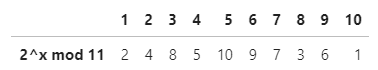
\includegraphics[width=6.9cm]{potenzen.png} \\

Lösung: \\
Es gilt: $A \equiv g^a \tmod p$, also: $ 5 \equiv 2^a \tmod 11$. Aus der Tabelle lesen wir $a = 4$ ab. Der gemeinsame Schlüssel ist dann $K \equiv B^a \equiv 8^4 \equiv 4 \tmod 11$
 \bigskip \stepcounter{y}
 
\newpage

\textbf{RSA} \bigskip

\textbf{A\arabic {y}:}   \\
Bob wählt p , q  und Verschlüsselungsexponent e. Warum ist e ein
zulässiger Verschlüsselungsexponent? Wie heißt der öffentliche, wie der private Schlüssel von Bob?
Alice will an Bob die Nachricht n verschlüsselt übermitteln.  
Welche Zahl schickt sie an Bob? Wie entschlüsselt Bob die Nachricht?

a.  p = 3, q = 11,  e = 7, n = 6. \quad
b.  p = 7, q = 11, e = 47, n = 2 \\

Lösung: \\
a. $m = p \cdot q = 33, \tilde{m} = (p-1)(q-1) = 20$, $\ggT(e,\tilde{m}) = \ggT(7,20) = 1$. Also ist
$e$ gültiger Verschlüsselungsexponent. Für den Entschlüsselungsexponenten $d$ muss gelten:
$\overline{d} = \dfrac{\overline{1}}{\overline{7}}$ in $\mathbb{Z}_{20}$. In diesem Fall können wir 
$d$ durch Hinschauen bestimmen. Wir suchen die Zahl, die mit 7 multipliziert bei Division durch 20 den Rest 1 ergibt. Also $d = 3$. \\
Der öffentliche Schlüssel ist $(33,7)$, der private Schlüssel ist $(33,3)$. \\
Alice verschlüsselt die Nachricht $n=10$: $N \equiv n^e \equiv 6^7 \equiv 30 \tmod 33$
(Nebenrechnung dazu: $6^1, 6^2, 6^4 \equiv 6, 3, 9 \tmod 33$).\\
Bob entschlüsselt die Nachricht $N=30$: $n \equiv N^d \equiv 30^3  \equiv 6 \tmod 33$
(Nebenrechnung dazu: $30^1, 30^2 \equiv -3, 9 \tmod 33$). \\

b. $m = p \cdot q = 77, \tilde{m} = (p-1)(q-1) = 60$, $\ggT(e,\tilde{m}) = \ggT(47,60) = 1$. Also ist
$e$ gültiger Verschlüsselungsexponent. Für den Entschlüsselungsexponenten $d$ muss gelten:
$\overline{d} = \dfrac{\overline{1}}{\overline{47}}$ in $\mathbb{Z}_{60}$. Wir ermitteln $d$ mit dem Erweiterten Euklidschen Algorithmus durch Lösen der diophantischen Gleichung $47x + 60y = 1$. \\
\begin{lstlisting}
    a    b    q    r    x    y
   60   47    1   13  -18   23
   47   13    3    8    5  -18
   13    8    1    5   -3    5
    8    5    1    3    2   -3
    5    3    1    2   -1    2
    3    2    1    1    1   -1
    2    1    2    0    0    1
\end{lstlisting}
Der öffentliche Schlüssel ist $(77,47)$, der private Schlüssel ist $(77,23)$. \\
Alice verschlüsselt die Nachricht $n=2$: $N \equiv n^e \equiv 2^{47} \equiv 18 \tmod 77$
(Nebenrechnung dazu: $2^1, 2^2, 2^4,2^8,2^{16},2^{32}\equiv 2, 4, 16,25,9,4 \tmod 77$).\\
Bob entschlüsselt die Nachricht $N=18$: $n \equiv N^d \equiv 18^{23}  \equiv 2 \tmod 77$
(Nebenrechnung dazu: $18^1, 18^2, 18^4, 18^8, 18^{16} \equiv 18,16,25,9,4 \tmod 77$).


\end{document}
